\documentclass[12pt,a4paper]{report}
\usepackage[utf8]{inputenc}
\usepackage{amsmath}
\usepackage{amsfonts}
\usepackage{amssymb}
\usepackage{makeidx}
\usepackage{graphicx}
\usepackage{algorithm,listings}
\usepackage{algpseudocode}

\newcommand{\mytitle}{AI-Powered Surveillance Vehicle:
Real-Time Object Detection with ESP32-CAM}

\usepackage[left=4cm,right=2cm,top=3cm,bottom=3cm]{geometry}
\newcommand{\mySpace}{0.5cm}
\newcommand{\mySpaceHalf}{0.5cm}
\usepackage{tikz}
\usetikzlibrary{shapes,arrows,positioning}
\renewcommand{\contentsname}{\centering Contents}
\usepackage{hyperref}

  

\begin{document}
\clearpage
	\newgeometry{left=2cm, right=2cm, top=3cm, bottom=3cm}
	\begin{titlepage}

    \centering
    %{\Huge \mytitle \fontsize{24}{28.8}\selectfont
     %\fontfamily{ptm}\selectfont}\\

{\Huge AI-Powered Surveillance Vehicle:\\[0.5cm]Real-Time Object Detection with ESP32-CAM \fontsize{24}{28.8}\selectfont 
\fontfamily{ptm}\selectfont}\\
    
    
\vspace{\mySpace}
%	\begin{center}
 %   		{\fontsize{24}{28.8}\selectfont  {Gesture-Nav: Hand-Controlled Virtual Mouse}}
%	\end{center}
    \large \textit{By}\\
\vspace{\mySpace}
    {\Large TAMAL MALLIK ( CSE21099 / 759 ) \\
    \vspace{0.1cm}
    AVISHEK MONDAL ( CSE21019 / 679 ) \\
    \vspace{0.1cm}
    SOUVIK BAIDYA ( CSE21088  / 748 ) \\
    \fontsize{18}{22}\selectfont \fontfamily{ptm}\selectfont
\vspace{\mySpace}}
    \begin{center}
        
\includegraphics[width=0.5\textwidth]{iiitk_logo} %img
    \end{center}
    {\Large \textit{Bachelor Thesis submitted to}\\
    \vspace{\mySpaceHalf}
    Indian Institute of Information Technology Kalyani \\ \vspace{\mySpaceHalf}
	 \textit{for the partial fulfillment of the degree of}\\ \vspace{\mySpaceHalf}

{\bfseries %bolding
	 Bachelor of Technology \\ 
	 in \\
	 Computer Science and Engineering\\ \vspace{\mySpaceHalf}
	  November, 2024 \fontsize{18}{22}}\selectfont \fontfamily{ptm}\selectfont}
    \vspace*{\fill}
\end{titlepage}
\restoregeometry


%	\author{Tamal Mallick , Avishek Mondal, Souvik Baidya}
%	\title{GestureNav: Hand-Controlled Virtual Mouse }
%	\maketitle
%	GestureNav: Hand Controlled Virtual Mouse
%
	\newpage
	\pagenumbering{roman}
	\chapter*{\centering Certificate}
\label{sec:engack}
This is to certify that the synopsis entitled \textbf{"\mytitle "} is being submitted by Tamal Mallick,
 (\textbf{Enrollment No: CSE/21099/759 }), Avishek Mondal (\textbf{Enrollment No: CSE21019/679} and Souvik Baidya (\textbf{Enrollment No: CSE21088/748}, B.Tech., Indian Institute of Information Technology Kalyani, India, for the partial fulfillment of the requirements for the registration of the degree of Bachelor of Technology is an original research work carried by them under my supervision. The synopsis has fulfilled all the requirements as per the regulation of IIIT Kalyani and in my opinion, has reached the standards needed for submission. The works, techniques, and results presented have not been submitted to any other university or Institute for the award of any other degree or diploma.
\\
\\
\\
\\
\\
\\
\\
\\
\textbf{Dr. Anirban Lakshman}  \\ 
$Assistant Professor \\  
Department of Mathematics\\
Indian Institute of Information Technology Kalyani\\
Kalyani-741235, W.B., India.
$
\cleardoublepage



	\chapter*{\centering Declaration}
\label{sec:engack}
We hereby declare that the work being submitted in this thesis entitled,\textbf{"\mytitle "}, submitted to Indian Institute of Information Technology, Kalyani in partial fulfillment for the award of the degree of Bachelor of Technology in Computer Science and Engineering during the period from July, 2024 to November 2024 under the supervision of Dr. Anirban Lakshman, Department of Computer Science and Engineering, Indian Institute of Information Technology Kalyani, West Bengal 741235, India, does not contain any classified information. 
\\
\\
\\
\\
\\
\\
\\
$
\\
\textbf{Tamal Mallick} \\
Enrollment No.: CSE/21099/759\\
Indian Institute of Information Technology Kalyani\\
Kalyani - 741235, W.B., India.
\\
\\
\\
\\
\textbf{Avishek Mondal}\\
Enrollment No.: CSE/21019/679\\
Indian Institute of Information Technology Kalyani\\
Kalyani - 741235, W.B., India.
\\
\\
\\
\\
\textbf{Souvik Baidya}\\
Enrollment No.: CSE21088/748\\
Indian Institute of Information Technology Kalyani\\
Kalyani - 741235, W.B., India.
$

\cleardoublepage
	
			\newpage
			\chapter*{\centering Acknowledgement}
We hereby acknowledge our deep sense of gratitude to our supervisor Dr. Anirban Lakshman, Department of Mathematics, Indian Institute of Information Technology Kalyani, for providing us with adequate facilities, ways, and means by which we are able to do this work. We express our sincere gratitude to him, his valuable time, insightful suggestions, and constant support have been indispensable for our progress.\\
\\
	Finally, we would also like to thank our friends, college faculties and family members who in one way or another helped us in doing this work.\\
\\
\\
\\
\\
\\
$
\\
\textbf{Tamal Mallick} \\
Enrollment No.: CSE/21099/759\\
Indian Institute of Information Technology Kalyani\\
Kalyani - 741235, W.B., India.
\\
\\
\\
\\
\textbf{Avishek Mondal}\\
Enrollment No.: CSE/21019/679\\
Indian Institute of Information Technology Kalyani\\
Kalyani - 741235, W.B., India.
\\
\\
\\
\\
\textbf{Souvik Baidya}\\
Enrollment No.: CSE21088/748\\
Indian Institute of Information Technology Kalyani\\
Kalyani - 741235, W.B., India.
$


\cleardoublepage
	\chapter*{\centering Abstract }
\label{Abstract}
This project presents the development of a wireless surveillance vehicle equipped with an integrated \textbf{ESP32-CAM camera}, designed for \textbf{real-time monitoring} and \textbf{security applications} \cite{esp32cam}. The vehicle uses the \textbf{ESP32-CAM development board} for live video streaming, enabling \textbf{remote surveillance} with high accessibility. Movement control is achieved using the \textbf{L298N motor driver}, offering \textbf{precise navigation} capabilities. The system further incorporates \textbf{YOLO-based real-time object detection}, enabling the automatic identification and tracking of objects within the vehicle's environment \cite{yolov10}. \\

A user-friendly \textbf{mobile and desktop application} has been developed for \textbf{remote control}, enhancing the flexibility of operation. The project demonstrates a \textbf{compact and cost-effective solution} for surveillance, suitable for \textbf{security, military, and industrial monitoring} applications. In its current form, the vehicle provides \textbf{real-time video streaming} and \textbf{object detection}, while \textbf{future work} aims to integrate \textbf{AI-driven autonomous navigation} and \textbf{advanced object recognition} for improved decision-making and automated operation \cite{homl}.






\cleardoublepage



		\tableofcontents

			\chapter*{\centering Abbreviations Used }
		\label{Abbreviations Used}
		
		

\begin{table}[ht]
\centering
\begin{tabular}{|c|l|}
\hline
\textbf{Abbreviation} & \textbf{Full Form} \\ \hline
ESP32-CAM & ESP32 Camera Module \\ \hline
L298N & Dual H-Bridge Motor Driver \\ \hline
YOLO & You Only Look Once (Object Detection Model) \\ \hline
SAR & Search and Rescue \\ \hline
STEM & Science, Technology, Engineering, and Mathematics \\ \hline
IoT & Internet of Things \\ \hline
Gzip & GNU zip (Compression Algorithm) \\ \hline
API & Application Programming Interface \\ \hline
ML & Machine Learning \\ \hline
AI & Artificial Intelligence \\ \hline
CNN & Convolutional Neural Network \\ \hline
LiDAR & Light Detection and Ranging \\ \hline
4G/5G & Fourth/Fifth Generation Wireless Technology \\ \hline
LoRa & Long Range Radio \\ \hline
GPS & Global Positioning System \\ \hline
PWM & Pulse Width Modulation \\ \hline
ROS & Robot Operating System \\ \hline
VGA & Video Graphics Array \\ \hline
SNR & Signal-to-Noise Ratio \\ \hline
DRL & Deep Reinforcement Learning \\ \hline
GAN & Generative Adversarial Networks \\ \hline
\end{tabular}
\caption{List of Abbreviations Used in the Project}
\label{tab:abbreviations}
\end{table}




	\renewcommand{\thesection}{\arabic{section}}
	
	\newpage
		\pagenumbering{arabic}
	{\vfill \chapter*{\centering \vfill Chapter 1 \vfill}\vfill}
	\thispagestyle{empty}
	\newpage

	\label{Introduction}
	\section{Introduction}

Surveillance technologies have become increasingly essential in enhancing security and monitoring capabilities across various sectors, including residential, commercial, military, and industrial applications \cite{esp32cam}. Traditional systems, such as fixed cameras and drones, have limitations in mobility, affordability, and real-time object detection \cite{anymal}. These shortcomings make them less effective in scenarios requiring dynamic, on-the-go surveillance.

In response to these challenges, this project focuses on the development of a \textbf{wireless surveillance vehicle} equipped with an \textbf{ESP32-CAM} module for \textbf{real-time video streaming} and \textbf{machine learning} for \textbf{object detection} \cite{esp32cam}. The objective is to create a compact, cost-effective solution that allows for efficient and flexible surveillance in various environments. By integrating \textbf{YOLO (You Only Look Once)}, a state-of-the-art real-time object detection algorithm, the vehicle can automatically identify and track objects, providing enhanced situational awareness \cite{yolov10}.

Furthermore, the project aims to enable \textbf{remote control} through a \textbf{desktop or web application}, allowing the user to operate the vehicle seamlessly from a distance. The incorporation of \textbf{Gzip compression} and \textbf{multi-threading} techniques ensures optimal performance, even in low-resource environments \cite{homl}. This system is designed to be scalable, with future goals including the integration of \textbf{AI-based autonomous navigation} for fully autonomous operations.

The development of this vehicle highlights the growing need for affordable, scalable, and intelligent surveillance solutions that can adapt to various monitoring environments, from security and military applications to industrial use cases \cite{robotsearch}.


	\label{Problem Statement}
	\subsection{Problem Statement }
The advent of surveillance technologies has significantly enhanced security and monitoring capabilities. However, traditional systems, such as fixed cameras and expensive drones, often lack mobility and affordability. These limitations are particularly evident in scenarios requiring stealth, flexibility, and versatility, which are crucial in real-time surveillance applications \cite{robotsearch}. There is a growing need for a \textbf{compact}, \textbf{cost-effective} surveillance vehicle capable of \textbf{real-time video streaming} for effective remote monitoring.

To address these challenges, the goal of this project was to \textbf{design and 3D print} the necessary components, develop the circuits, and assemble the system for seamless operation. In addition, we integrated \textbf{YOLO 10 machine learning} for \textbf{real-time object detection}, ensuring smooth and efficient surveillance while maintaining control via a \textbf{desktop application} \cite{yolov10}.


\label{Objective}  
\subsection{Objective}  

The main objective of this project is to develop a \textbf{wireless surveillance vehicle} equipped with \textbf{real-time video streaming} and \textbf{machine learning} for \textbf{object detection}. The specific objectives are as follows:  

\subsubsection*{Component Design and Integration}  
\begin{itemize}  
    \item \textbf{3D printing} and precisely fitting the vehicle's components, ensuring compatibility and a compact design for effective operation \cite{3dprinting}.  
    \item Designing and assembling the \textbf{circuitry} to support the communication between the vehicle's components, including the ESP32-CAM, motor drivers, and other essential modules \cite{circuitdesign}.  
\end{itemize}  

\subsubsection*{Firmware and Software Development}  
\begin{itemize}  
    \item Writing the \textbf{ESP32 firmware} to enable video streaming, control the vehicle's movement, and interface with external systems \cite{esp32cam}.  
    \item Developing and implementing \textbf{APIs} for \textbf{external control} of the vehicle through desktop and web applications.  
\end{itemize}  

\subsubsection*{System Optimization}  
\begin{itemize}  
    \item Implementing \textbf{Gzip compression} to reduce video streaming latency and improve the system's responsiveness while maintaining low memory consumption.  
    \item Ensuring smooth, real-time video streaming and \textbf{machine learning predictions} with \textbf{multi-threading} to optimize performance \cite{homl}.  
\end{itemize}  

\subsubsection*{Control and User Interface}  
\begin{itemize}  
    \item Developing \textbf{easy-to-use keyboard shortcuts} for controlling the vehicle’s movements and video streaming functionalities.  
    \item Providing an accessible interface through \textbf{desktop and web applications} to enable intuitive control of the surveillance vehicle from remote locations.  
\end{itemize}  

\subsubsection*{Machine Learning Integration}  
\begin{itemize}  
    \item Integrating \textbf{YOLO (You Only Look Once)} machine learning model for \textbf{real-time object detection} on the vehicle's live camera feed, enabling automatic identification and tracking of objects \cite{yolov10}.  
    \item Ensuring \textbf{smooth real-time prediction} and object detection performance on the device while maintaining minimal computational overhead through optimization techniques.  
\end{itemize}  

\subsubsection*{System Testing and Evaluation}  
\begin{itemize}  
    \item Conducting rigorous testing of the vehicle’s movement control, video streaming quality, and object detection accuracy in various operational environments.  
    \item Evaluating the overall performance and stability of the system, including response time, accuracy, and usability under real-world conditions.  
\end{itemize}  





	{\vfill \chapter*{\centering \vfill Chapter 2 \vfill}\vfill}
	\thispagestyle{empty}
	\newpage
\label{Literature Review}
\section{Literature Review}

This section presents a review of existing research related to autonomous and wireless surveillance robots, highlighting key developments and their relevance to our project. The studies reviewed explore various technologies, including robot autonomy, IoT-enabled systems, and the integration of wireless communication for surveillance tasks.

\subsection{Autonomous Multi-Robot Search for Hazardous Source}
\label{Autonomous Multi-Robot Search for Hazardous Source}
\textbf{Authors:} Branko Ristic, Daniel Angley, Bill Moran, Jennifer L. Palmer \\ \\
\textbf{Published In:} Autonomous Robots, 2021. \\ \\
\textbf{Overview:} This research presented cognitive algorithms for robots to search and locate hazardous sources in turbulent environments. The robots utilized Bayesian estimation for efficient pathfinding, enabling them to function autonomously. The study highlighted centralized fusion architecture and scalable robot formations, optimizing their movement and sensing strategies \cite{robotsearch}. \\ \\
\textbf{Relevance to Project:} The exploration of autonomous systems for hazardous areas underlines the importance of reliable sensors and communication. While our spy vehicle does not operate autonomously, the integration of video streaming and real-time controls lays the groundwork for future autonomous capabilities, inspired by such research.

\subsection{ANYmal: Robotic Systems for Challenging Environments}
\label{ANYmal: Robotic Systems for Challenging Environments}
\textbf{Authors:} Dr. Péter Fankhauser, Prof. Dr. Marco Hutter \\ \\
\textbf{Published In:} Robotics and Automation Magazine, 2017. \\ \\
\textbf{Overview:} Developed at ETH Zurich, ANYmal is a four-legged robot designed to operate in hazardous terrains such as industrial platforms and mines. Equipped with advanced cameras, lidar, and torque motors, ANYmal autonomously performs search, rescue, and surveillance tasks. It operates seamlessly in dusty, wet, and uneven environments, demonstrating remarkable adaptability and autonomy \cite{anymal}. \\ \\
\textbf{Relevance to Project:} Although ANYmal represents a complex system, its ability to perform surveillance in challenging environments directly correlates with our spy vehicle's design goal: operating effectively in confined or dangerous zones with video feedback.

\subsection{Key Takeaways}
\label{Key Takeaways}
The following key takeaways are drawn from the reviewed literature:

\begin{itemize}
    \item \textbf{Wireless Communication and IoT:} The adoption of Wi-Fi and IoT technologies like ESP32-CAM allows for efficient remote operation, a key feature of our spy vehicle \cite{esp32cam}.
    \item \textbf{Customizable and Lightweight Designs:} Studies highlight the growing importance of 3D printing in creating scalable, lightweight robots, aligning with the fabrication methods used in our vehicle \cite{3dprinting}.
    \item \textbf{Autonomous Navigation Potential:} While our spy vehicle is manually controlled, the research on autonomous systems inspires potential future enhancements, such as integrating AI for navigation and obstacle avoidance.
\end{itemize}

This literature survey highlights the advancements in surveillance robotics that serve as a foundation and inspiration for our project.






	{\vfill \chapter*{\centering \vfill Chapter 3 \vfill}\vfill}
	\thispagestyle{empty}
	\newpage
	\label{System Design and Components}
	\section{System Design and Components}
	\label{Workflow Overview}
	\subsection{Workflow Overview}

The system is designed to function seamlessly through three core stages \cite{esp32cam, circuitdesign, yolov10}:

\begin{enumerate}
    \item \textbf{Input:} Commands are sent by the user via a remote interface, typically an internet-enabled device such as a smartphone or computer. These commands control the vehicle's movement (forward, backward, left, right) and trigger additional functionalities like activating video streaming \cite{iot}.
    
    \item \textbf{Processing:} The ESP32-CAM module acts as the processing unit. It receives user commands, interprets them into control signals, and processes the live video feed captured by its camera. Simultaneously, it sends motor control signals to the L298N motor driver for precise movement and navigation \cite{esp32cam, circuitdesign}.
    
    \item \textbf{Output:} 
    \begin{itemize}
        \item The ESP32-CAM streams live video directly to the user's interface over Wi-Fi, providing real-time visual feedback \cite{esp32cam}.
        \item The motor driver controls the vehicle's movement based on user commands, ensuring smooth navigation and obstacle avoidance \cite{circuitdesign}.
        \item Real-time object detection is performed on the live video stream from the ESP32-CAM using the YOLO model, automatically identifying and tracking objects in the environment \cite{yolov10}.
    \end{itemize}
\end{enumerate}

This workflow ensures a cohesive interaction between hardware components, software logic, machine learning, and user control.











\label{List of Components}
\subsection{List of Components}

\begin{enumerate}
    \item \textbf{ESP32-CAM Development Board:}
    \begin{itemize}
        \item \textbf{Functionality:} Serves as the core processing unit for the vehicle, enabling both live video streaming and wireless communication.
        \item \textbf{Specifications:}
        \begin{itemize}
            \item Camera: OV2640 (supports JPEG/BMP/Grayscale formats).
            \item Connectivity: Wi-Fi (802.11 b/g/n), Bluetooth (BLE).
            \item Power: Operates at 5V with low power consumption.
        \end{itemize}
        \item \textbf{Role in System:} Captures video, processes user commands, and transmits data to and from the remote device. \\ 
\begin{figure}[H]
    \centering
    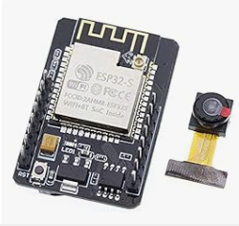
\includegraphics[width=0.5\textwidth]{espCam}
    \caption{ESP -CAM Development Board}
    \label{fig:espCam}
\end{figure}
 
    \end{itemize}



    \item \textbf{L298N Motor Driver Module:}

    \begin{itemize}
        \item \textbf{Functionality:} Controls the vehicle's motors for precise movement.
        \item \textbf{Specifications:}
        \begin{itemize}
            \item Input Voltage: 5-35V.
            \item Output Current: 2A per channel (dual H-bridge).
            \item PWM Control: Enables speed and direction control for two motors.
        \end{itemize}
        \item \textbf{Role in System:} Receives motor control signals from the ESP32-CAM and adjusts motor operation accordingly.\\


\begin{figure}[H]
    \centering
    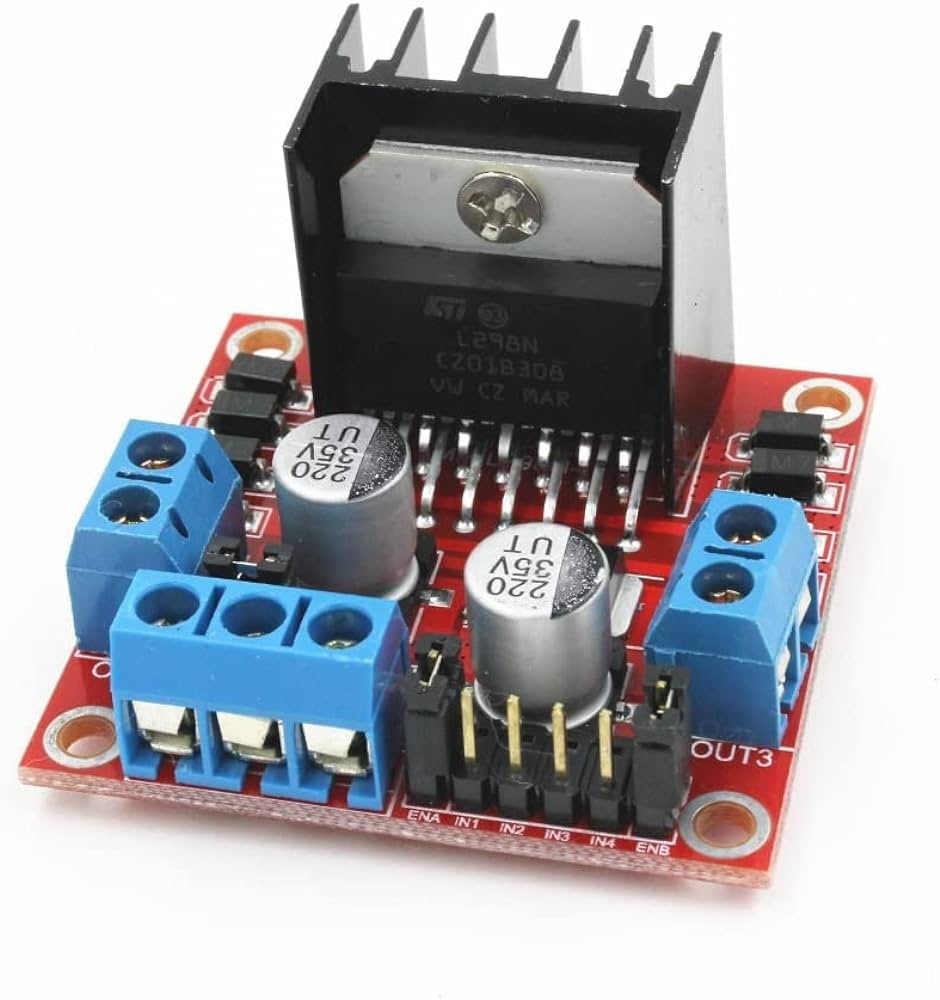
\includegraphics[width=0.5\textwidth]{l298n}
    \caption{L298N Motor Driver}
    \label{fig:l298n}
\end{figure}

    
    \end{itemize}

    \item \textbf{Boost and Buck Converter:}
    \begin{itemize}
        \item \textbf{Functionality:} Stabilizes the power supply to all components by stepping up or stepping down the voltage as needed.
        \item \textbf{Specifications:}
        \begin{itemize}
            \item Input Range: 5-12V.
            \item Output Range: Configurable to supply stable 5V for ESP32-CAM and 12V for motor operation.
        \end{itemize}
        \item \textbf{Role in System:} Ensures consistent and reliable power to prevent system interruptions.
        
        
\begin{figure}[H]
    \centering
    \begin{minipage}{0.45\textwidth}
        \centering
        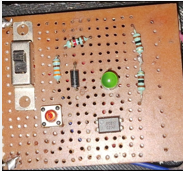
\includegraphics[width=\textwidth]{powerCircuit}  % Boost Converter Image
        \caption{Boost Converter Circuit}
        \label{fig:powerCircuit}
    \end{minipage} \hfill
    \begin{minipage}{0.45\textwidth}
        \centering
        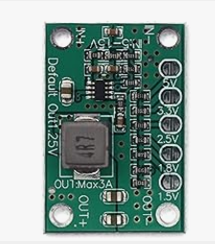
\includegraphics[width=\textwidth]{buckConverter}  % Buck Converter Image
        \caption{Buck Converter Circuit}
        \label{fig:buckConverter}
    \end{minipage}
\end{figure}        
        
    \end{itemize}

    \item \textbf{Chassis and Motors:}
    \begin{itemize}
        \item \textbf{Chassis:}
        \begin{itemize}
            \item Custom-designed and 3D-printed for lightweight and durable operation.
            \item Includes mounting points for the camera, motor driver, and other components.
        \end{itemize}
        \item \textbf{Motors:}
        \begin{itemize}
            \item Type: DC motors with high torque for all-terrain mobility.
            \item Integrated with encoders for better control and feedback.
        \end{itemize}
        
\begin{figure}[H]
    \centering
    \begin{minipage}{0.45\textwidth}
        \centering
        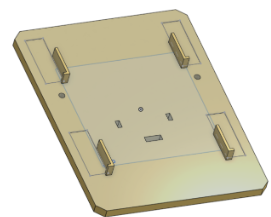
\includegraphics[width=\textwidth]{base}  % First Image (Base)
        \caption{Chassis}
        \label{fig:base}
    \end{minipage} \hfill
    \begin{minipage}{0.45\textwidth}
        \centering
        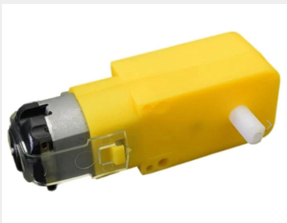
\includegraphics[width=\textwidth]{bodMotor}  % Second Image (BOD Motor)
        \caption{High Torque BOD Motor}
        \label{fig:bodMotor}
    \end{minipage}
\end{figure}
        
        
    \end{itemize}



    \item \textbf{Power Supply:}
    \begin{itemize}
        \item \textbf{Battery:} A 10,000mAh Li-ion rechargeable battery with a 12V output powers the system.
        \item \textbf{Role in System:} Provides the energy needed to run motors, ESP32-CAM, and auxiliary components, ensuring a runtime of approximately 2 hours under continuous operation.
        
\begin{figure}[H]
    \centering
    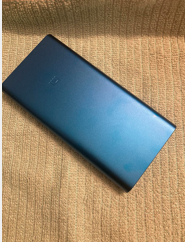
\includegraphics[width=0.5\textwidth]{powerBank}
    \caption{Power Bank}
    \label{fig:powerBank}
\end{figure}        
        
    \end{itemize}

    \item \textbf{Additional Components:}
    \begin{itemize}
        \item \textbf{Servo Motor Modules:}
        \begin{itemize}
            \item Quantity: 3 modules for actuating specific functionalities, such as camera rotation or storage mechanisms.
        \end{itemize}
        \item \textbf{Connectors and Holders:}
        \begin{itemize}
            \item Wheel-to-body connectors, wire holders, and clamps designed for secure assembly and ease of maintenance.
        \end{itemize}
    \end{itemize}
    
\begin{figure}[H]
    \centering
    \begin{minipage}{0.30\textwidth}
        \centering
        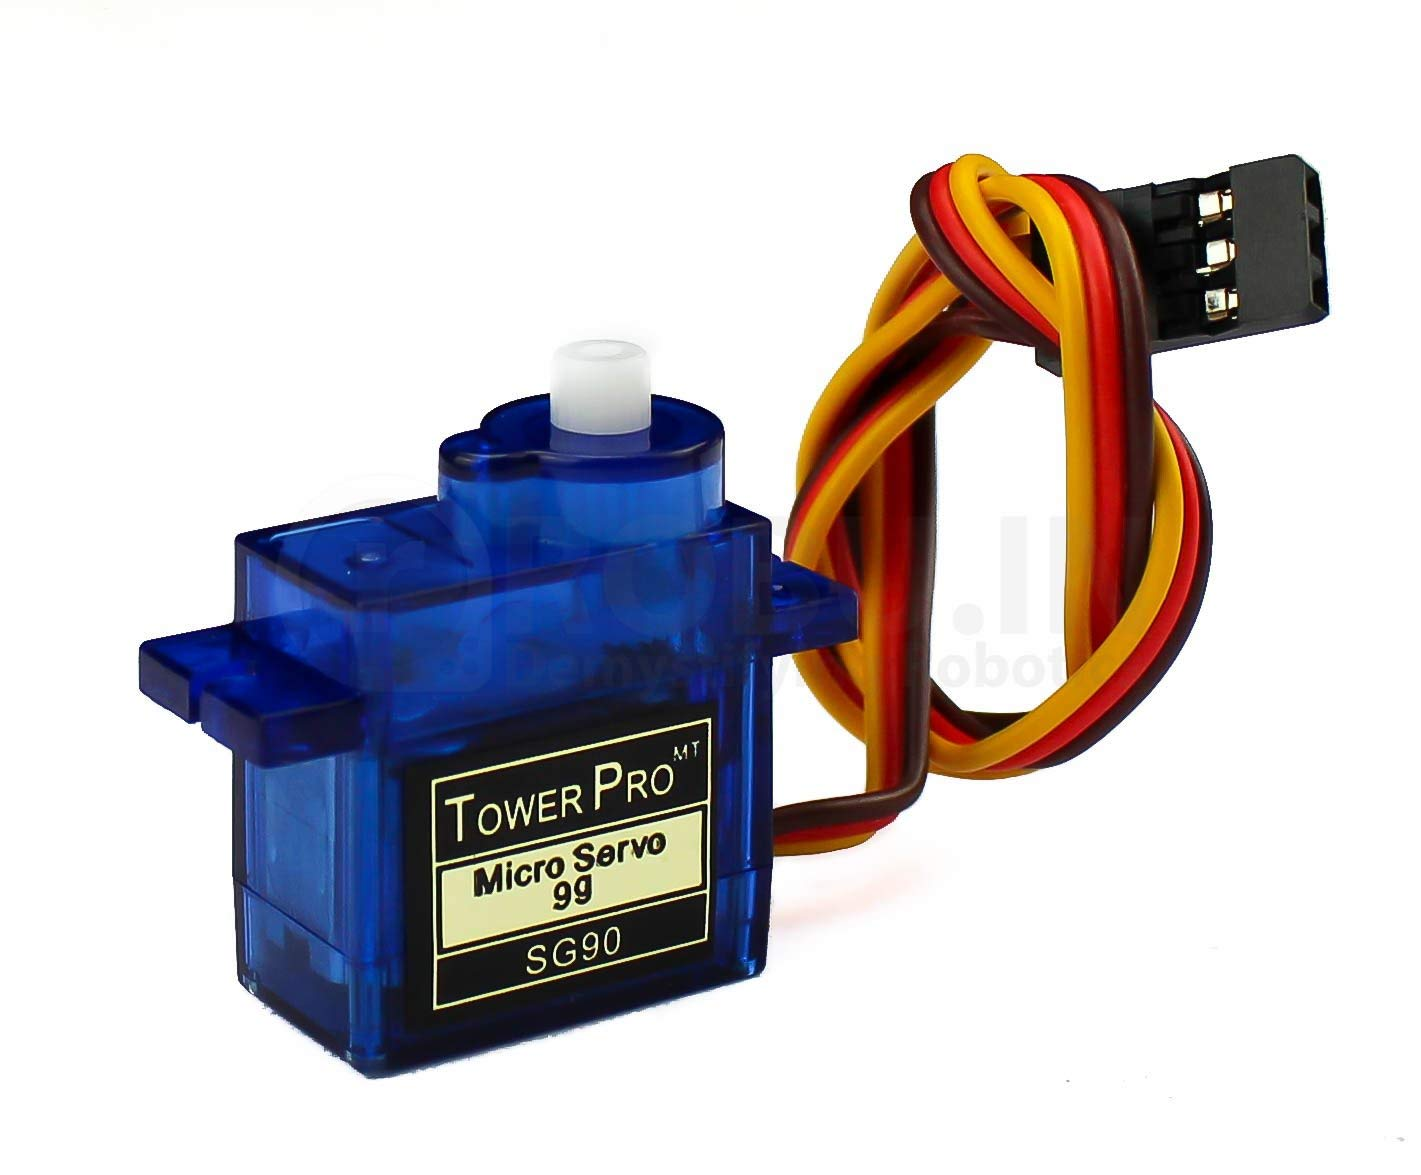
\includegraphics[width=\textwidth]{s90}  % S90 Servo Motor Image
        \caption{Servo Motor}
        \label{fig:s90}
    \end{minipage} \hfill
    \begin{minipage}{0.30\textwidth}
        \centering
        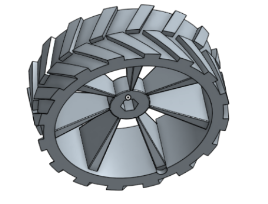
\includegraphics[width=\textwidth]{wheel}  % 3D Printed Wheel Image
        \caption{Wheel}
        \label{fig:wheel}
    \end{minipage} \hfill
    \begin{minipage}{0.3\textwidth}
        \centering
        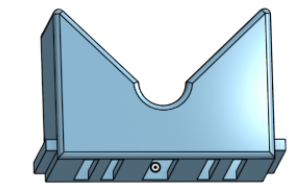
\includegraphics[width=\textwidth]{espHolder}  % 3D Printed Wheel Connector Image
        \caption{ESP32 Holder}
        \label{fig:espHolder}
    \end{minipage}
\end{figure}    
    
    
\end{enumerate}





\label{Circuit Design}
\subsection{Circuit Design}

The circuit forms the backbone of the surveillance vehicle, integrating the ESP32-CAM, motor driver, and power system to ensure seamless operation \cite{esp32cam, circuitdesign}. Key details are as follows:

\begin{enumerate}
    \item \textbf{ESP32-CAM Connections:}
    \begin{itemize}
        \item GPIO pins interface with the L298N motor driver to transmit control signals \cite{esp32cam}.
        \item Camera pins connect to the onboard OV2640 camera module for video processing \cite{esp32cam}.
    \end{itemize}
    
    \item \textbf{Motor Driver Connections:}
    \begin{itemize}
        \item The L298N receives PWM signals from the ESP32-CAM for speed and direction control \cite{circuitdesign}.
        \item Outputs O1 and O2 drive the left motor, while O3 and O4 drive the right motor \cite{circuitdesign}.
    \end{itemize}
    
    \item \textbf{Power Distribution:}
    \begin{itemize}
        \item The boost converter supplies 12V for the motor driver and motors \cite{circuitdesign}.
        \item The buck converter steps down the voltage to 5V for the ESP32-CAM \cite{circuitdesign}.
    \end{itemize}
    
    \item \textbf{Additional Circuit Features:}
    \begin{itemize}
        \item Servo motor connections for additional functionalities.
        \item Voltage regulators to prevent component damage from power surges \cite{circuitdesign}.
    \end{itemize}




\begin{figure}[H]
    \centering
    \begin{minipage}{0.45\textwidth}
        \centering
        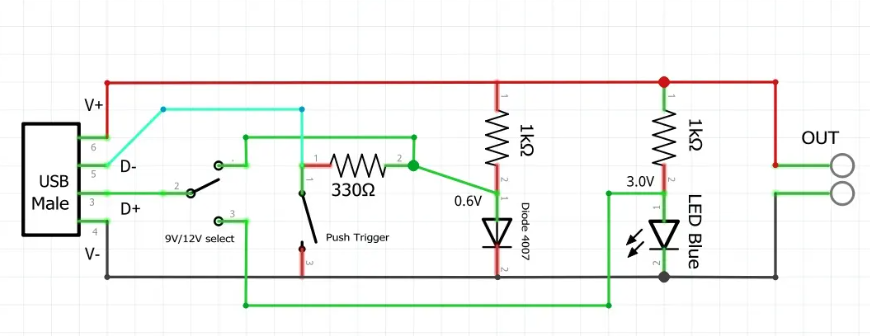
\includegraphics[width=\textwidth]{usbPowerbank}  % First Image (Base)
        \caption{12 V Activator Circuit Diagram for Power Bank}
        \label{fig:base}
    \end{minipage} \hfill
    \begin{minipage}{0.45\textwidth}
        \centering
        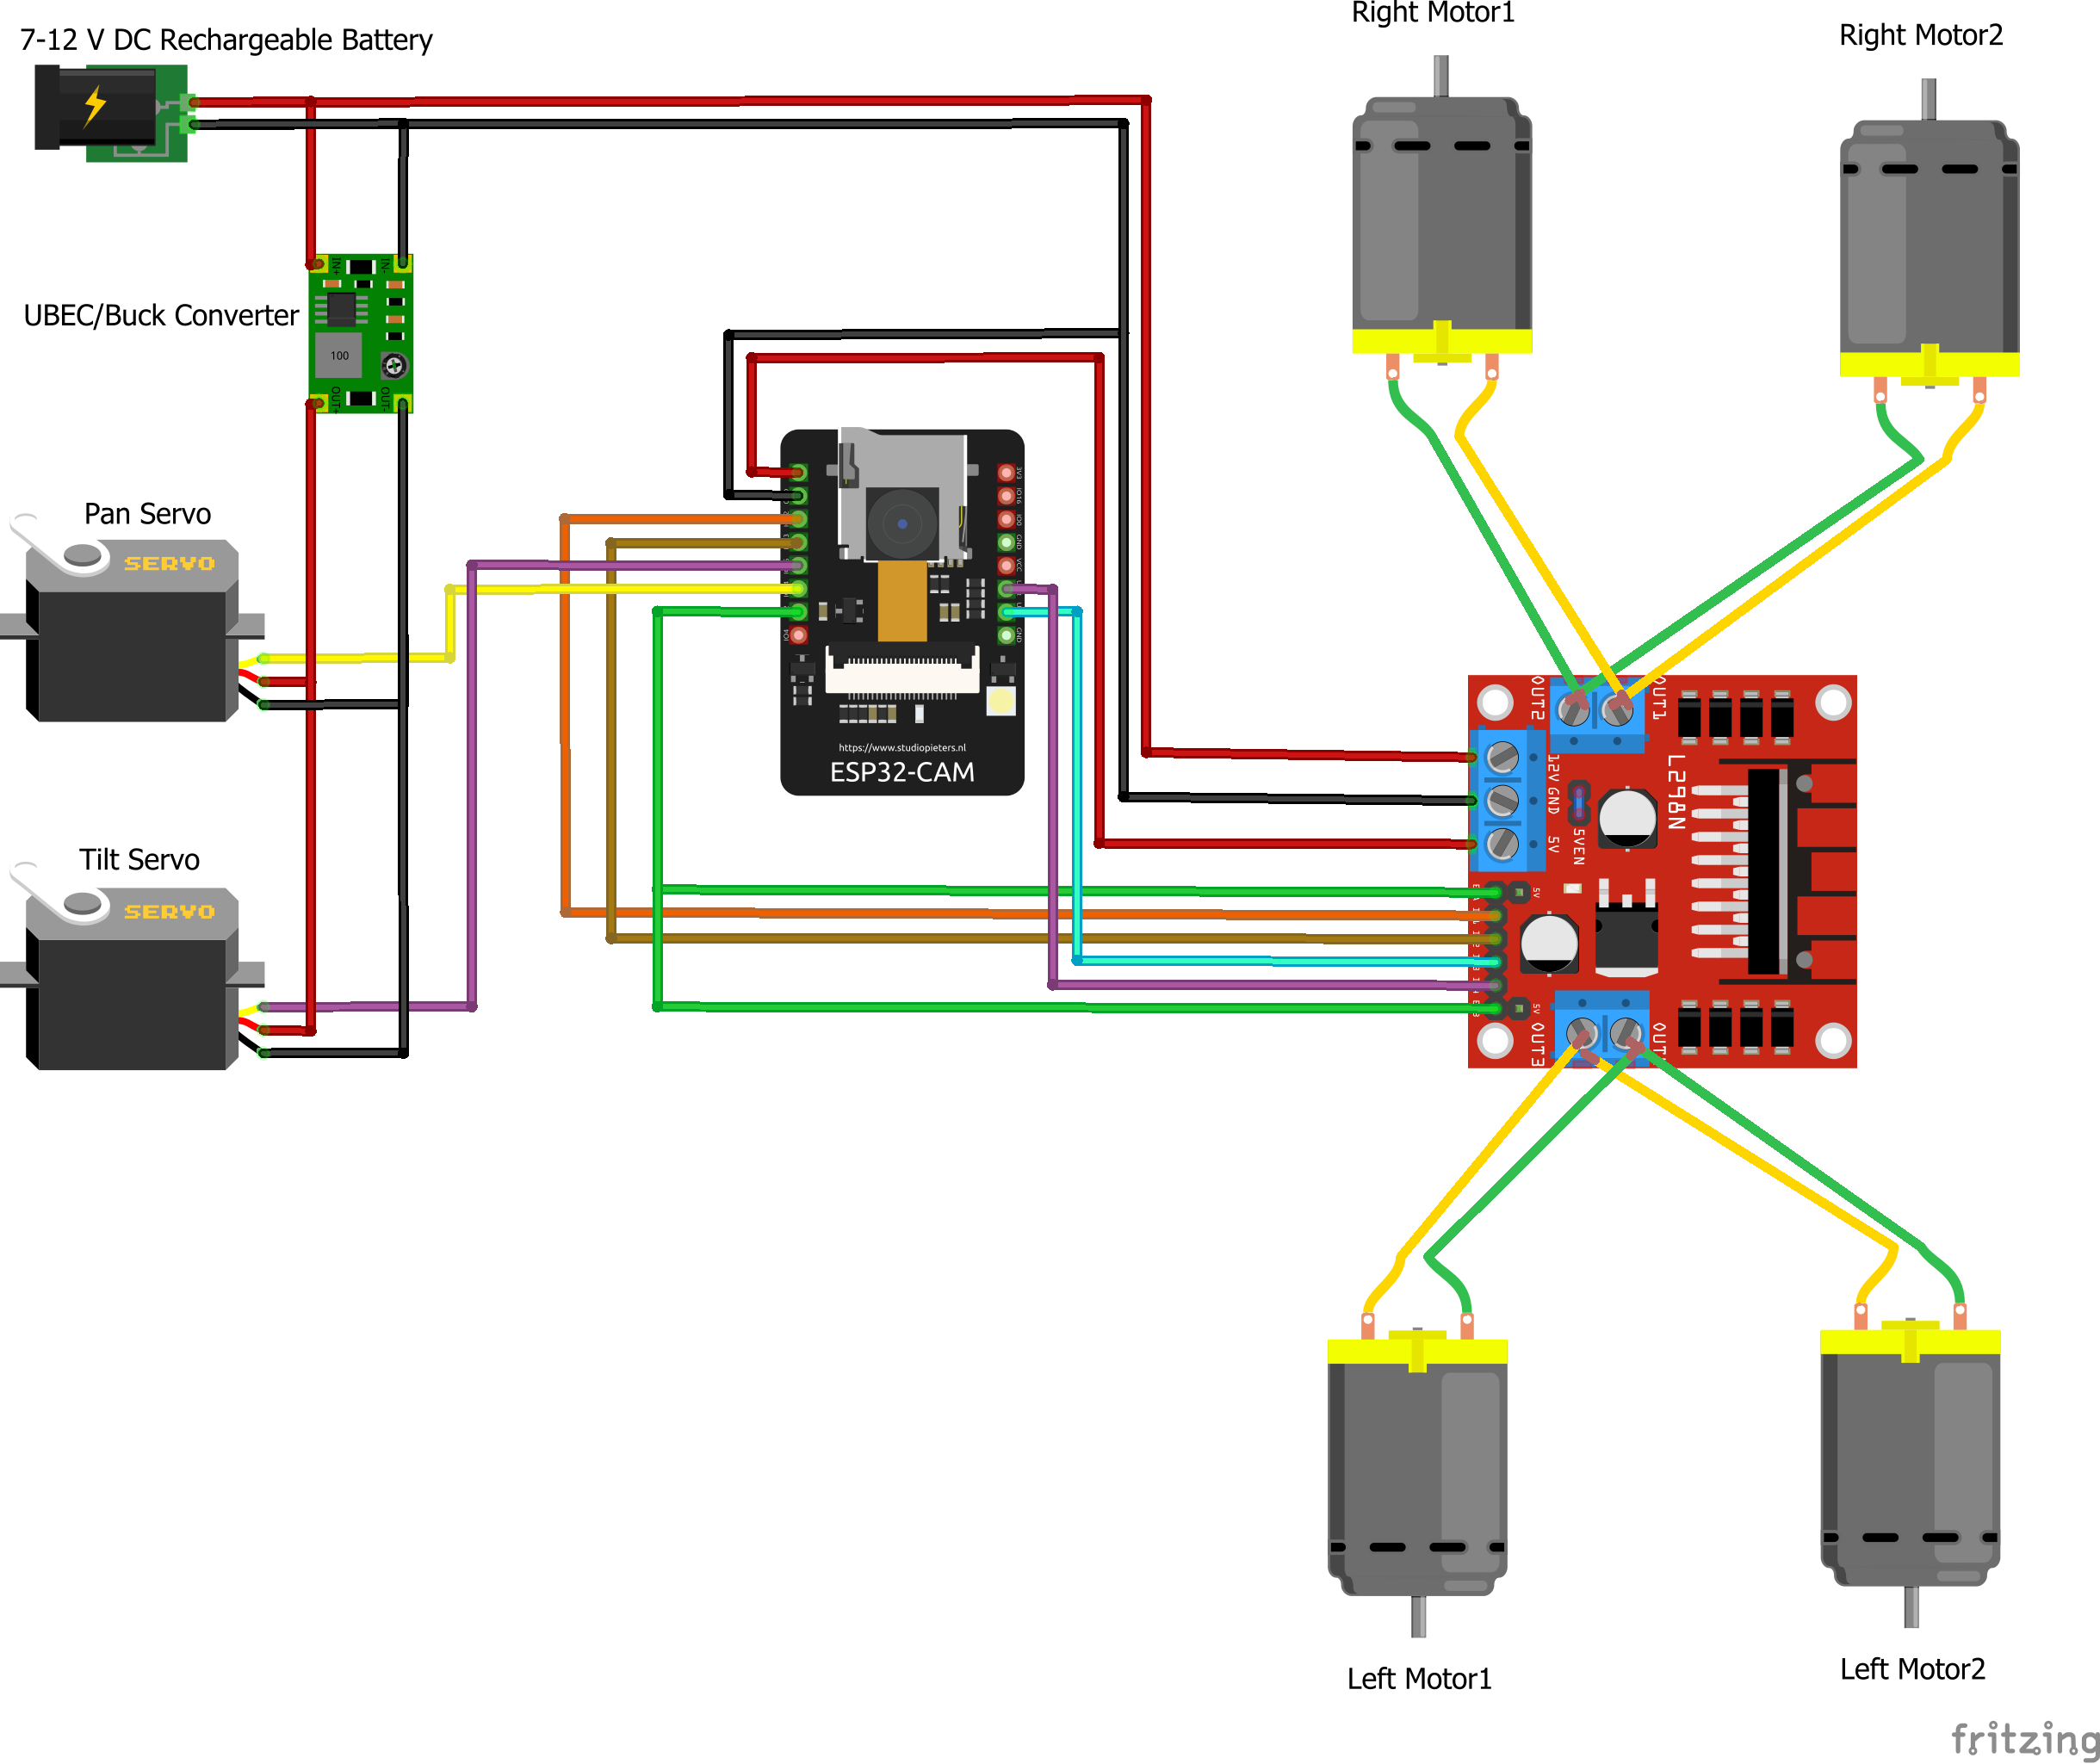
\includegraphics[width=\textwidth]{circuitDiagram}  % Second Image (BOD Motor)
        \caption{Vehicle Circuit Diagram}
        \label{fig:circuitDiagram}
    \end{minipage}
\end{figure}    
    
\end{enumerate}





	{\vfill \chapter*{\centering \vfill Chapter 4 \vfill}\vfill}
	\thispagestyle{empty}
	\newpage
	\label{Implementation}
	\section{Implementation}
\label{Hardware Assembly}
\subsection{Hardware Assembly}

\begin{enumerate}
    \item \textbf{Chassis Design:} \\
     The chassis and its associated components, including wheels and connectors, were entirely designed and fabricated by our team. Each part was carefully modeled using CAD software to meet the specific requirements of the spy vehicle, ensuring optimal functionality and durability \cite{3dprinting, circuitdesign}.
    \begin{itemize}

        \item \textbf{Custom Design:} The chassis, wheels, and wheel-to-body connectors were designed using CAD software to meet the vehicle’s specific operational requirements. The design was optimized for stability, lightweight construction, and compactness, ensuring easy mobility and adaptability to various terrains \cite{circuitdesign}.
        \item \textbf{3D Printing:} 
        \begin{itemize}
            \item The chassis and other components were 3D-printed using PLA (Polylactic Acid) material, chosen for its strength, precision, and lightweight properties \cite{3dprinting}.
            \item The wheel and connector designs incorporated additional reinforcements to withstand continuous movement and vibrations during operation \cite{3dprinting}.
        \end{itemize}
        \item \textbf{Assembly:} 
        \begin{itemize}
            \item Each 3D-printed part was meticulously aligned and assembled to form the complete chassis. Screws, adhesives, and clamps were used to secure the components, ensuring durability and preventing misalignment during vehicle operation \cite{3dprinting}.
        \end{itemize}
    \end{itemize}


    
    
\item \textbf{Wiring:} \\
A critical step in hardware assembly is establishing the electrical connections between components to ensure seamless functionality. The wiring setup consists of power connections, control connections, and wire management, all of which follow the circuit design outlined earlier \cite{iot, circuitdesign, robotsearch}.

\begin{itemize}
    \item \textbf{Power Connections:}
    \begin{itemize}
        \item A boost converter steps up the voltage to 12V to power the motors \cite{circuitdesign}.
        \item A buck converter regulates the voltage to 5V for the ESP32-CAM module \cite{circuitdesign}.
    \end{itemize}
    
    \item \textbf{Control Connections:}
    \begin{itemize}
        \item The ESP32-CAM is connected to the motor driver via GPIO pins to send control signals for motor direction and speed \cite{esp32cam}.
        \item Ultrasonic sensors and servo motors are interfaced with additional GPIO pins for obstacle detection and other functionalities \cite{iot, robotsearch}.
    \end{itemize}
    
    \item \textbf{Wire Management:}
    \begin{itemize}
        \item Wire holders and clamps were used to organize and secure the wiring, reducing clutter and preventing electrical interference \cite{robotsearch}.
    \end{itemize}
\end{itemize}



\end{enumerate}


\label{Software Development}
\subsection{Software Development}

The software development phase focused on configuring the ESP32-CAM module for real-time video streaming and programming motor control logic for precise movement of the spy vehicle. Both functionalities were integrated using the Arduino IDE, which provides a robust platform for programming and debugging microcontroller-based systems \cite{esp32cam}.


\begin{enumerate}

\item \textbf{Wheel Control Logic:}
\begin{itemize}
    \item \textbf{Pin Configuration:}
    \begin{itemize}
        \item \textbf{Motor A1 ,A2 (Left Motors):} Controlled by IN1 and IN2, connected to GPIO 12 and GPIO 13, respectively.
        \item \textbf{Motor B1, B2 (Right Motors):} Controlled by IN3 and IN4, connected to GPIO 14 and GPIO 15, respectively.
        \item \textbf{Enable Pins:} ENA and ENB are connected to ground, enabling the motor drivers and allowing the enable pins to control motor speed.
    \end{itemize}
    \item \textbf{PWM for Speed Variation:} PWM (Pulse Width Modulation) signals are used to dynamically adjust the motor speeds. This enables smooth transitions between different movement commands.
\end{itemize}


\item \textbf{Servo Control Logic}
\begin{itemize}
    \item \textbf{Horizontal Movement:} A servo motor connected to GPIO 2 is used to control the horizontal (X-axis) movement of the camera, with a range of 0 to 180 degrees.
    \item \textbf{Vertical Movement:} A servo motor connected to GPIO 4 is used to control the vertical (Y-axis) movement of the camera, with a range of 0 to 180 degrees.
    \item \textbf{Function:} These servo motors adjust the camera's direction, allowing it to rotate along the X and Y axes for full 180-degree coverage.
\end{itemize}


\item \textbf{Flash Light Control Logic}
\begin{itemize}
    \item \textbf{Control:} GPIO 4 is used to send PWM signals to control the built-in flashlight.
    \item \textbf{Function:} The PWM signal allows the flashlight to be turned on or off and adjusts its intensity based on the signal's duty cycle.
\end{itemize}


    
\item \textbf{Video Streaming Configuration:}
\begin{itemize}
    \item \textbf{Wi-Fi Server Setup:} The ESP32-CAM is programmed to act as a Wi-Fi server. Once powered on, the module connects to a local Wi-Fi network or operates in access point mode, allowing the user to connect directly.
    \item \textbf{Data Transmission:} The video feed is captured in JPEG format to optimize bandwidth usage. JPEG compression reduces the size of image files, ensuring smooth and low-latency streaming even with moderate network speeds.
    \item \textbf{Stream Access:} The video stream is accessible via a unique URL provided by the ESP32-CAM once it connects to the network. This stream can be viewed on any browser-compatible device \cite{iot}.
\end{itemize}

    
\item \textbf{Remote Control and Interface Design:}
\begin{itemize}
    \item A desktop user interface (UI) was developed using PyQt5 to access the video stream and control the remote vehicle over Wi-Fi via API endpoints.
    \item The UI allows users to control the vehicle's movement, including:
    \begin{itemize}
        \item Forward, backward, and combinations of wheel movements.
        \item Servo movements for camera adjustments.
    \end{itemize}
    \item The interface also enables:
    \begin{itemize}
        \item Viewing the live video feed and predictions from the machine learning model.
        \item Controlling the flashlight's intensity.
    \end{itemize}
    \item To enhance usability, multi-threading and keyboard shortcuts were implemented for seamless monitoring and control of the vehicle.
\end{itemize}


\end{enumerate}


\label{Object Detection using Machine Learning}
\subsection{Object Detection using Machine Learning}
\begin{enumerate}
\item The video stream was accessed from port 81/stream using the OpenCV library, with a resolution set to 800x600 from the ESP32-CAM module to ensure a balance between video quality and processing speed. This allowed for smooth streaming and efficient handling of frames for further processing \cite{esp32cam}.
\item Machine learning integration was achieved using the YOLO v10 (You Only Look Once) model, specifically the YOLOv10n variant, which is optimized for faster object detection. YOLOv10n was applied over each frame of the live video stream to perform real-time object detection \cite{yolov10}.
\item Once an object was detected in each frame, bounding boxes were drawn around the identified objects. These boxes were accompanied by labels and confidence scores, which represent the accuracy of the prediction. This labeling and annotation were performed using OpenCV, enabling visual feedback of detected objects and their categories \cite{homl}.
\item To optimize the system for real-time performance, the object detection pipeline was fine-tuned to provide fast and accurate predictions. The YOLO model was configured for optimal processing speed, ensuring that predictions could be made in real time with minimal latency, making the system capable of detecting objects quickly and accurately even in dynamic environments \cite{robotsearch}.

   
    \begin{figure}[H]
    \centering
    \begin{minipage}{0.30\textwidth}
        \centering
        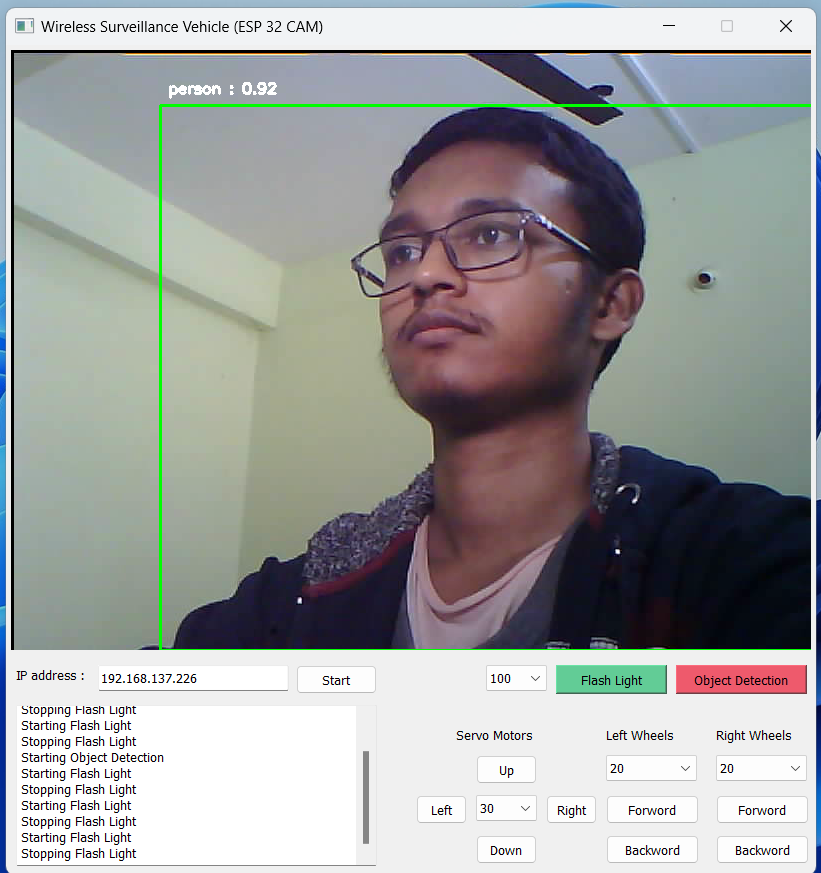
\includegraphics[width=\textwidth]{person}  % S90 Servo Motor Image
        \caption{Detecting Person}
        \label{fig:person}
    \end{minipage} \hfill
    \begin{minipage}{0.30\textwidth}
        \centering
        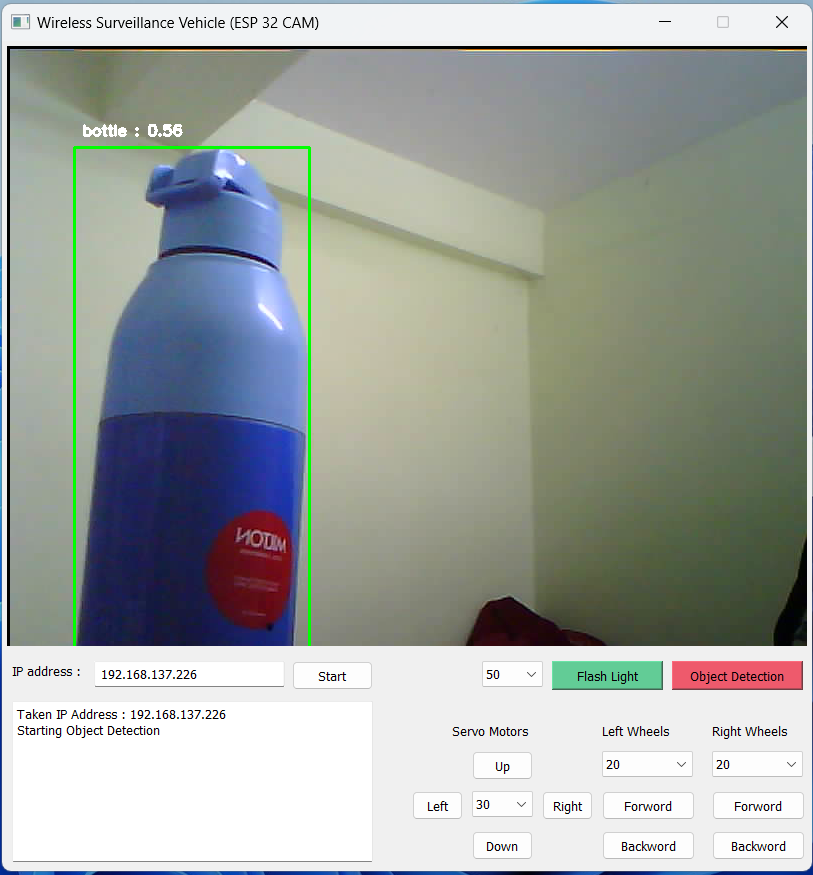
\includegraphics[width=\textwidth]{bottle}  % 3D Printed Wheel Image
        \caption{Detecting Bottle}
        \label{fig:bottle}
    \end{minipage} \hfill
    \begin{minipage}{0.3\textwidth}
        \centering
        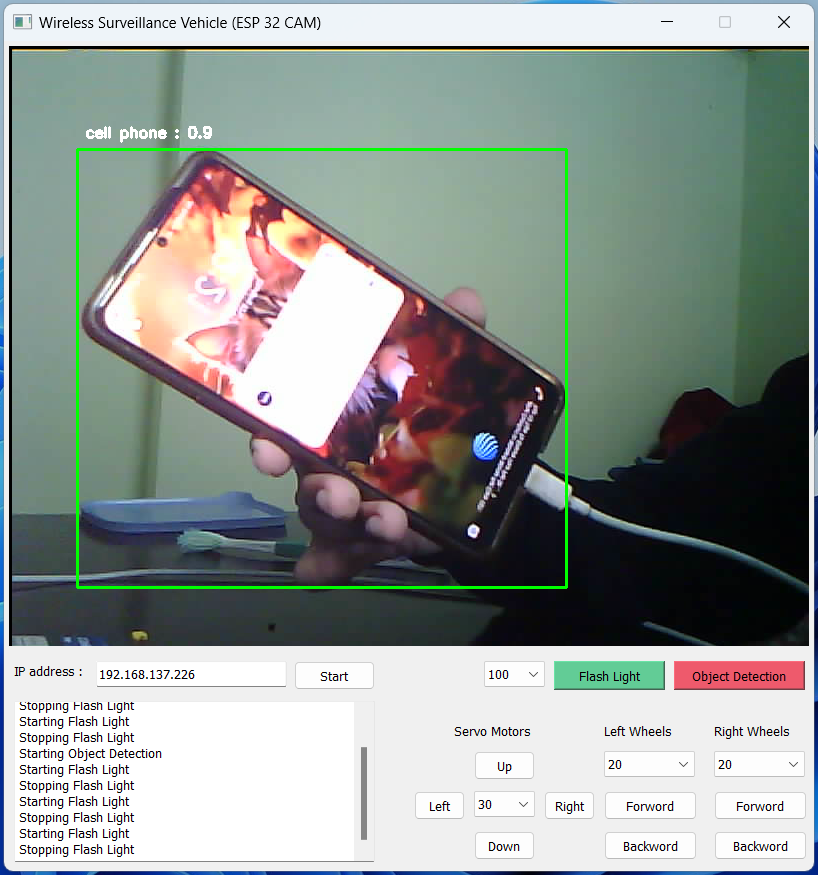
\includegraphics[width=\textwidth]{phone}  % 3D Printed Wheel Connector Image
        \caption{Detecting Cell Phone}
        \label{fig:phone}
    \end{minipage}
\end{figure}  
\end{enumerate}



\label{Challenges and Solutions}
\subsection{Challenges and Solutions}

Throughout the development and assembly process, several challenges were encountered. The following table highlights key issues and the corresponding solutions:

\begin{enumerate}
    \item \textbf{Video Quality and Lagging Issues:} 
    \begin{itemize}
        \item Solution: Reduced the resolution and frame rate to optimize bandwidth usage while maintaining acceptable clarity for smooth video streaming.
    \end{itemize}


    \item \textbf{3D Printing Dimensional Errors:}
    \begin{itemize}
        \item Solution: Iteratively adjusted CAD designs based on the initial prints to achieve precise dimensions, ensuring proper fit and assembly.
    \end{itemize}

    \item \textbf{Component Heating Issues:}
    \begin{itemize}
        \item Solution: Added heat sinks to high-power components like the motor driver to effectively dissipate heat and prevent overheating during prolonged use.
    \end{itemize}

    \item \textbf{Wi-Fi Connectivity Limitations:}
    \begin{itemize}
        \item Solution: Positioned the ESP32-CAM’s antenna optimally to maximize signal strength and minimize interference, ensuring stable communication over Wi-Fi.
    \end{itemize}

    \item \textbf{Power Fluctuations due to Initial Motor Start:}
    \begin{itemize}
        \item Solution: The initial motor start-up required a high current, causing voltage drops below 4.5V, which led to the ESP32-CAM rebooting. To mitigate this, the upper limit for the current drawn by the four motors was capped to 75\%, as the wheels almost don't move below 25\%, and voltage drops below 4.5V at 80-90\%. This adjustment ensures that the ESP32-CAM consistently receives a stable 5V supply and avoids power-related resets.
    \end{itemize}
    
        \item \textbf{Improvement in YOLO Model Prediction Speed:}
    \begin{itemize}
\item Solution: Implemented multi-threading to allow faster YOLO model predictions, enabling real-time object detection with improved accuracy and minimal delay \cite{yolov10,homl}
    \end{itemize}
\end{enumerate}











	{\vfill \chapter*{\centering \vfill Chapter 5 \vfill}\vfill}
	\thispagestyle{empty}
	\newpage
	\label{Testing and Performance Evaluation}
	\section{Testing and Performance Evaluation}
	
\label{Test Scenarios}
\subsection{Test Scenarios}
To ensure the spy vehicle meets the desired performance standards, extensive testing was conducted under various conditions. The tests focused on evaluating core functionalities such as video streaming, motor control, and overall system reliability. Key scenarios include:

\begin{enumerate}
    \item \textbf{Video Latency and Wi-Fi Range Testing}
    \begin{itemize}
        \item \textbf{Indoor Testing:}
        \begin{itemize}
            \item The vehicle was operated in a standard room-sized indoor environment with several obstructions, including walls and furniture.
            \item Wi-Fi signal strength and video latency were measured at different distances (up to 20 meters).
            \item Results were analyzed to determine the impact of obstructions on streaming quality and control responsiveness.
        \end{itemize}
        \item \textbf{Outdoor Testing:}
        \begin{itemize}
            \item Testing was performed in an open outdoor area with minimal obstructions to maximize Wi-Fi range.
            \item The vehicle’s ability to stream video and receive commands at distances up to 30 meters was evaluated.
            \item Environmental factors such as wind and sunlight glare were noted to assess their impact on video clarity.
        \end{itemize}
    \end{itemize}




\item \textbf{ESP32 Webserver API Endpoints Testing}
   \begin{itemize}

    \item \textbf{1. Testing Wheels}
    \\ The API allows testing of the wheels by controlling their direction and speed. The direction is determined by the \textit{control} parameter, and the speed is specified as a percentage via the \textit{value} parameter.
    \begin{figure}[H]
        \centering
        \begin{minipage}{0.45\textwidth}
            \centering
            \includegraphics[width=\textwidth]{wheelTest1}  % Image 1 for testing wheels
            \caption{Testing Left Wheel}
            \label{fig:wheelTest1}
        \end{minipage} \hfill
        \begin{minipage}{0.45\textwidth}
            \centering
            \includegraphics[width=\textwidth]{wheelTest2}  % Image 2 for testing wheels
            \caption{Testing Right Wheel}
            \label{fig:wheelTest2}
        \end{minipage}
    \end{figure}

    \item \textbf{2. Testing Servo Motors}
    \\ The servo motors are controlled by specifying the type of servo (horizontal or vertical) and the degree of rotation. The \textit{control} parameter specifies the servo type, and the \textit{value} parameter sets the rotation degree.
    \begin{figure}[H]
        \centering
        \begin{minipage}{0.45\textwidth}
            \centering
            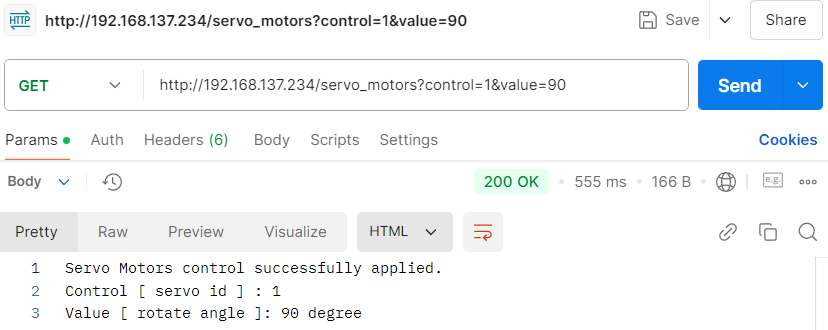
\includegraphics[width=\textwidth]{servoMotorTest1}  % Image 1 for testing servo motors
            \caption{Testing Horizontal Servo Motor}
            \label{fig:servoMotorTest1}
        \end{minipage} \hfill
        \begin{minipage}{0.45\textwidth}
            \centering
            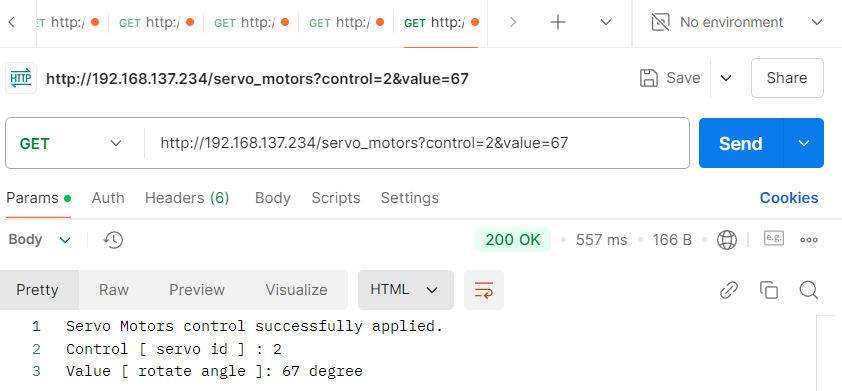
\includegraphics[width=\textwidth]{servoMotorTest2}  % Image 2 for testing servo motors
            \caption{Testing Vertical Servo Motor}
            \label{fig:servoMotorTest2}
        \end{minipage}
    \end{figure}

    \item \textbf{3. Testing Flashlight}
    \\ The flashlight is tested by turning it on or off using the \textit{control} parameter, while the \textit{value} parameter adjusts the light's intensity, expressed as a percentage.
    \begin{figure}[H]
        \centering
        \begin{minipage}{0.45\textwidth}
            \centering
            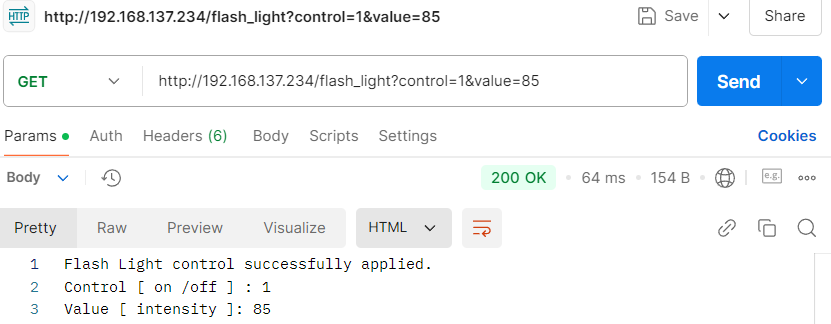
\includegraphics[width=\textwidth]{flashlightTest1}  % Image 1 for testing flashlight
            \caption{Testing Flashlight On}
            \label{fig:flashlightTest1}
        \end{minipage} \hfill
        \begin{minipage}{0.45\textwidth}
            \centering
            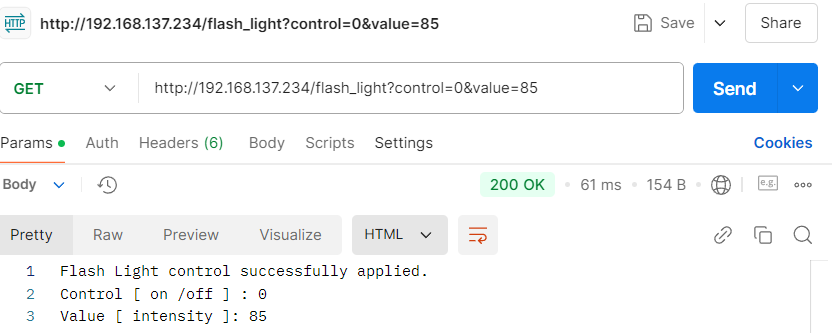
\includegraphics[width=\textwidth]{flashlightTest2}  % Image 2 for testing flashlight
            \caption{Testing Flashlight Off}
            \label{fig:flashlightTest2}
        \end{minipage}
    \end{figure}

   \end{itemize}




    
   
    
    
    
    
        \item \textbf{Motor Speed and Direction Control}
    \begin{itemize}
        \item \textbf{Smooth Surface Testing:}
        \begin{itemize}
            \item The vehicle’s movement was tested on smooth surfaces, such as tiled and wooden floors, to ensure consistent speed and directional accuracy.
            \item Commands for forward, backward, left, and right movements were executed repeatedly to measure response times.
        \end{itemize}
        \item \textbf{Rough Surface Testing:}
        \begin{itemize}
            \item Tests were conducted on uneven terrains, including gravel, grass, and sand, to evaluate the vehicle’s adaptability.
            \item The torque of the motors and the durability of the chassis were monitored under these conditions.
        \end{itemize}
    \end{itemize}

    \item \textbf{Obstacle Navigation and Stability Testing}
    \begin{itemize}
        \item The ultrasonic sensor’s obstacle detection capabilities were tested by placing objects at various distances.
        \item The system's responsiveness to avoid collisions and maintain stability during sudden changes in direction was analyzed.
    \end{itemize}

    \item \textbf{Battery Performance Testing}
    \begin{itemize}
        \item The battery’s endurance was tested by operating the vehicle continuously in both idle and active states.
        \item Power consumption was monitored while streaming video, moving motors, and running sensors simultaneously.
    \end{itemize}
\end{enumerate}







\label{Observations and Metrics}
\subsection{Observations and Metrics}

Based on the above test scenarios, the following key observations and metrics were recorded:

\begin{enumerate}
    \item \textbf{Video Latency:}
    \begin{itemize}
        \item Average latency of 250ms was observed under optimal conditions, with minor variations during extended operation or at the edge of the Wi-Fi range.
        \item \textbf{Indoors:} Latency increased slightly (up to 300ms) when multiple obstructions were present.
        \item \textbf{Outdoors:} Latency remained stable at approximately 250ms, ensuring smooth video feedback.
    \end{itemize}
    
    \item \textbf{Wi-Fi Range:}
    \begin{itemize}
        \item \textbf{Indoors:} Effective range was 15-20 meters, depending on wall thickness and material.
        \item \textbf{Outdoors:} The system maintained connectivity and video streaming up to 30 meters, with no significant drop in performance.
    \end{itemize}
    
    \item \textbf{Motor Speed and Direction:}
    \begin{itemize}
        \item On smooth surfaces, the vehicle achieved consistent speeds with rapid directional changes.
        \item On rough surfaces, speed reduced by approximately 20%, but torque remained sufficient to handle the terrain without stalling.
    \end{itemize}
    
    \item \textbf{Obstacle Detection:}
    \begin{itemize}
        \item The ultrasonic sensor reliably detected obstacles within a 50cm range.
        \item The vehicle successfully stopped or adjusted its path in response to detected obstacles.
    \end{itemize}
    
    \item \textbf{Battery Life:}
    \begin{itemize}
        \item Continuous operation, including video streaming and motor activity, lasted approximately 2 hours.
        \item Idle operation extended battery life to 3 hours, highlighting the system’s power efficiency.
    \end{itemize}
\end{enumerate}



\label{Discussion of Results}
\subsection{Discussion of Results}

The test results demonstrated the reliability and efficiency of the spy vehicle’s design and functionality. Key observations include:

\begin{enumerate}
    \item \textbf{Video Streaming and Control:}
    \begin{itemize}
        \item The ESP32-CAM provided stable video streaming with low latency, ensuring effective surveillance in real time.
        \item Wi-Fi performance was satisfactory for both indoor and outdoor environments, with only minor limitations in highly obstructed areas.
    \end{itemize}
    
    \item \textbf{Mobility and Terrain Adaptability:}
    \begin{itemize}
        \item The L298N motor driver and DC motors enabled precise movement and adequate torque, ensuring the vehicle’s adaptability to different terrains.
        \item Despite slight speed reductions on rough surfaces, the system maintained stability and responsiveness.
    \end{itemize}
    
    \item \textbf{Power Efficiency:}
    \begin{itemize}
        \item The use of a buck converter ensured consistent power delivery to the ESP32-CAM, while the boost converter supported motor operations efficiently.
        \item The battery performance was within the expected range, supporting prolonged surveillance tasks without frequent recharges.
    \end{itemize}
    
    \item \textbf{Obstacle Navigation:}
    \begin{itemize}
        \item The ultrasonic sensor effectively complemented the manual control system, providing an additional layer of safety during operation.
        \item This functionality is particularly beneficial in environments where user visibility is limited or obstructed.
    \end{itemize}
\end{enumerate}










	{\vfill \chapter*{\centering \vfill Chapter 6 \vfill}\vfill}
	\thispagestyle{empty}
	\newpage
	\label{Applications}
	\section{Applications}

AI-Powered Surveillance Vehicle, equipped with real-time video streaming and wireless control, has several practical applications across multiple industries due to its mobility, affordability, and ease of use. Below are key areas where this technology can be deployed:

\begin{enumerate}
    \item \textbf{Military and Defence}
    \begin{itemize}
        \item \textbf{Reconnaissance and Surveillance:} The vehicle can be used in military operations for reconnaissance in hostile environments, providing real-time visual intelligence from a safe distance.
        \item \textbf{Border Patrol:} It can patrol and monitor borders, detecting unauthorized movements in remote areas without risking human lives.
    \end{itemize}
    
    \item \textbf{Industrial Monitoring}
    \begin{itemize}
        \item \textbf{Hazardous Area Inspections:} In industries like oil and gas or chemical plants, the vehicle can inspect dangerous areas, such as pipelines, reducing the need for personnel to enter high-risk zones.
        \item \textbf{Environmental Monitoring:} Equipped with environmental sensors, it can be used to monitor air quality, temperature, or potential gas leaks in hazardous industrial environments.
    \end{itemize}
        
    \item \textbf{Search and Rescue Operations (SAR)}
    \begin{itemize}
        \item \textbf{Disaster Response:} The vehicle can be deployed to disaster sites to assess damage, navigate through rubble, and provide real-time video footage, assisting in locating survivors.
        \item \textbf{Urban Search and Rescue:} It can navigate through confined spaces in urban environments, providing valuable footage to rescue teams.
    \end{itemize}
    
    \item \textbf{Environmental and Agricultural Monitoring}
    \begin{itemize}
        \item \textbf{Agriculture:} The vehicle can monitor crop health, detect pests, or assess soil conditions, reducing the need for manual inspections and improving operational efficiency.
        \item \textbf{Wildlife Monitoring:} It can be used in protected areas to monitor wildlife activities or track poaching without disturbing the ecosystem.
    \end{itemize}
    
    \item \textbf{Education and Training}
    \begin{itemize}
        \item \textbf{STEM Education:} The vehicle serves as an educational tool, offering hands-on experience for students studying robotics, wireless communication, and IoT technologies.
        \item \textbf{Professional Training:} It can also be used for training security professionals or disaster responders to control and interpret data from remote surveillance tools.
    \end{itemize}
\end{enumerate}







	{\vfill \chapter*{\centering \vfill Chapter 7 \vfill}\vfill}
	\thispagestyle{empty}
	\newpage
	\label{Conclusion and Future Scope}
	\section{Conclusion and Future Scope}


\label{Conclusion}
\subsection{Conclusion}
AI-Powered Surveillance Vehicle project successfully integrates wireless video streaming, motor control, and sensor integration into a compact and cost-effective surveillance solution. Its real-time video feed, mobility, and affordability make it highly versatile, with applications in military reconnaissance, industrial monitoring, public safety, and search and rescue operations.

AI-Powered Surveillance Vehicle goes beyond these applications. Future enhancements, such as autonomous navigation, AI-powered video analytics, extended communication ranges, and advanced sensors, could significantly improve its capabilities. Addressing these challenges will transform the spy vehicle into a more powerful tool for remote surveillance, broadening its utility in a wide range of industries.

As the project advances, future iterations of the spy vehicle are expected to become more autonomous, intelligent, and adaptable. The growing importance of IoT technologies and robotics ensures that the spy vehicle will play a key role in shaping the future of mobile surveillance systems.


\label{Future Scope}
\subsection{Future Scope}
AI-Powered Surveillance Vehicle project presents several avenues for future enhancements and applications. As technology evolves, additional features can be integrated to expand the vehicle's capabilities:

\begin{enumerate}
    \item \textbf{Autonomous Navigation:} 
    One key area for development is autonomous navigation. Currently, the vehicle relies on manual control via a remote interface. Incorporating sensors such as LiDAR or camera-based vision systems, along with machine learning algorithms, would allow the vehicle to navigate autonomously and avoid obstacles. This would enable tasks like autonomous patrols and hazardous area exploration without human intervention \cite{anymal}.
    
    \item \textbf{AI-Based Video Analytics:} 
    The integration of AI-powered video processing could enable the spy vehicle to analyze live video feeds in real-time. Features such as face recognition, motion detection, and object tracking could enhance security and surveillance capabilities, automating threat detection and reducing the need for constant human monitoring \cite{homl}.
    
    \item \textbf{Longer Range and Connectivity:} 
    Expanding the communication range to several kilometers using technologies like LoRa (Long Range Radio) or 4G/5G connectivity would extend the vehicle's operational range beyond the current 30 meters. This improvement would be valuable for large-area surveillance, border patrols, and more remote locations \cite{iot}.
    
    \item \textbf{Integration of Additional Sensors:} 
    To broaden its industrial applications, the vehicle could be equipped with additional sensors such as gas sensors, thermal cameras, and environmental monitoring tools. This would make it suitable for industrial inspections, chemical leak detection, and environmental monitoring in hazardous or difficult-to-reach areas \cite{3dprinting}.
    
    \item \textbf{Improved Power Efficiency:} 
    Enhancing battery life is crucial for extended missions, particularly in remote areas. Solar panels or more efficient power management systems could allow the vehicle to operate longer without frequent recharges, supporting continuous surveillance or extended-duration missions.
    
    
\item \textbf{Multi-Vehicle Coordination:} 
Developing a system for multiple vehicles to operate in coordinated swarms or fleets could expand the scope of the surveillance capabilities. This would enable the vehicles to cover a larger area simultaneously, provide redundancy in case of failure, and offer more comprehensive monitoring in complex environments. 

\item \textbf{Enhanced Data Security:} 
With the increasing reliance on wireless communication and real-time video feeds, ensuring data security is critical. Future versions of the vehicle could integrate advanced encryption and secure communication protocols to protect sensitive data from unauthorized access, ensuring that the surveillance system remains robust against cyber threats.

\item \textbf{Integration with Smart Cities:} 
The vehicle could be integrated into a smart city infrastructure, enabling it to contribute to urban surveillance, traffic management, and emergency response systems. By integrating with existing IoT-based city networks, it could provide real-time data to control centers, enhancing the efficiency of urban monitoring and response mechanisms.

\item \textbf{Advanced Machine Learning Algorithms:} 
As machine learning algorithms evolve, incorporating more advanced techniques such as deep reinforcement learning (DRL) and generative adversarial networks (GANs) could further enhance the vehicle's capabilities. DRL could be utilized for optimizing autonomous navigation and decision-making in dynamic environments, allowing the vehicle to adapt and learn from new situations without requiring predefined instructions. GANs could be explored for synthetic data generation, helping to train the vehicle’s AI system under diverse conditions, even when labeled data is scarce or difficult to obtain. These advancements would significantly improve the vehicle’s autonomy, accuracy in object detection, and real-time decision-making capabilities \cite{deepRL, gan}.



\end{enumerate}







	\newpage



%$\bibliographystyle{plain} $
\bibliographystyle{harvard}
\bibliography{references} 

	
\end{document}
